\documentclass[a4paper]{article}
\usepackage[margin=3cm]{geometry}
\usepackage[utf8]{inputenc}
\usepackage{cmbright}
\usepackage[hidelinks]{hyperref}
\usepackage{booktabs}
\usepackage[ngerman]{babel}
\usepackage{parskip}
\usepackage{graphicx}
\usepackage{minted}
\usepackage{pdflscape}
\usepackage{array}
\usepackage{tabulary}
\usepackage{multicol}
\usepackage{pgfgantt}
\usepackage{pgf-umlcd}
\usepackage{enumitem}

% Page breaks between sections
\let\oldsection\section
\renewcommand\section{\clearpage\oldsection}

% JIRA/Confluence shortcuts
\def\jiraurl{https://jira.keltec.ch/jira}
\def\confluenceurl{https://jira.keltec.ch/wiki}
\newcommand{\jiraissue}[1]{\href{\jiraurl/projects/EPJ/issues/EPJ-#1}{EPJ-#1}}
\newcommand{\fulljiraissue}[1]{EPJ-#1 (\url{\jiraurl/projects/EPJ/issues/EPJ-#1})}

% Tools
\newcommand{\tool}[2]{\emph{#1\footnote{\url{#2}}}}

\begin{document}
	\title{
		Projekt: kitovu \\
		\Large{Anforderungsspezifikation} \\[3em]
		
\includegraphics[width=20em]{../../img/logo/kitovu.jpg}
	}
	\author{
		Florian Bruhin \\ \url{florian.bruhin@hsr.ch} \and
		Méline Sieber \\ \url{meline.sieber@hsr.ch} \and
		Nicolas Ganz \\ \url{nicolas.ganz@hsr.ch} 
		}
	\date{\today}
	
	\maketitle

\section*{Änderungsgeschichte}

\begin{tabulary}{\linewidth}{llLl}
	\toprule
	Datum & Version & Änderung & AutorIn \\
	\midrule
	04.03.2018 & 1.0 & Dokument erstellt, Grundgerüst von Template übernommen, funktionale Anforderungen verfasst & Méline Sieber \\
	06.03.2018 & 1.1 & Überarbeitung & alle \\
  % FIXME
	08.03.2018 & 1.2 & Lektorat & Méline Sieber \\
	% 09.03.2018 & 2.0 & Abgabe & Florian Bruhin \\
	\bottomrule
\end{tabulary}
\pagebreak

\section{Einführung}
Dieses Dokument beschreibt Umfang und Funktionalitäten von \emph{kitovu}. Danach veranschaulicht diese Anforderungsspezifikation, wer \emph{kitovu} verwendet. Das erfolgt anhand von ``Use Cases'', einerseits in einem kurzen Format (\emph{brief}), andererseits in einer ausführlichen Beschreibung (\emph{fully dressed}). Entwürfe zur Benutzeroberfläche zeigen, wie wir uns vorstellen, wie \emph{kitovu} aussieht. Eine Domainanalyse zeigt wesentliche konzeptionelle Klassen und ihre Zusammenhänge auf. Weitere Anforderungen detaillieren, welche Qualitätsmerkmale und Schnittstellen verwendet werden sowie geltende Randbedingungen.

\subsection{Gültigkeitsbereich}
Die vorliegende Anforderungsspezifikation ist für das Engineering-Projekt im Frühlingssemester 2018 gültig. Falls dem Projekt grössere Veränderungen widerfahren, wird das Dokument dementsprechend angepasst. Umfassende Änderungen werden am Anfang des Dokuments protokolliert.

\subsection{Referenzen}
Die Anforderungsspezifikation ist eng mit der Domainanalyse und anderen Dokumenten verbunden. Die folgende Tabelle listet die wichtigsten Referenzen auf.

\begin{tabulary}{\linewidth}{Ll}
	Confluence & \url{\confluenceurl} \\
	Draw.io & \url{https://www.draw.io/} \\
	Github-Repository von \emph{kitovu} & \url{https://github.com/kitovu-bot/kitovu} \\
	JIRA	& \url{\jiraurl} \\
	Moodle & \url{https://moodle.hsr.ch} \\
	OpenHSR Connect & \url{https://github.com/openhsr/connect} \\
	Studentenportal & \url{https://studentenportal.ch/} \\
	Switch AAI (Authentication and Authorization Infrastructure)& \url{https://www.switch.ch/aai/} \\
\end{tabulary}

Beim Logo auf der Titelseite handelt es sich um eine stark überarbeitete Version eines GIFs (\url{https://www.animateit.net/details.php?image_id=8990}). Urheber und Copyright sind nicht auffindbar.

\pagebreak
\section{Allgemeine Beschreibung}

\subsection{Produktperspektive}
%<Produkt Perspektive beschreiben>

\subsection{Produktfunktion}
%<Allgemeine Beschreibung der Funktionen>
\emph{Kitovu} ist ein Client, der von verschiedenen Plattformen ausgewählte HSR-Unterrichtsmaterialien auf den eigenen Rechner synchronisiert, so dass sie lokal und offline verfügbar sind. Er läuft auf allen gängigen Betriebssystemen und funktioniert nicht nur für den HSR-Skripteserver, sondern ist auch erweiterbar für verschiedene Plattformen.

Unser Projekt bindet primär den Skripteserver ein. Der Kommandozeilen-basierte Client funktioniert mittels Profilen zu unterschiedlichen Plattformen (Moodle, Skripteserver, Studentenportal). Pro Profil sind Verbindungsdaten und eventuelle Login-Credentials im Client hinterlegt, alle Profile sind in einer Konfigurationsdatei gespeichert. Die Datei-Synchronisation erfolgt immer nur von Server zu Client, erfolgreiche und misslungene Datentransfers werden protokolliert. Ein rudimentäres GUI dient als Proof-of-Concept.

Pro Profil lässt sich Folgendes definieren:

\begin{itemize}
	\item welche Ordner/Dateien synchronisiert werden.
	\item welche Ordner/Dateien von der Synchronisation ausgeschlossen werden.
	\item wie mit Duplikaten/lokal bestehenden Dateien umgegangen wird.
\end{itemize}

\emph{Kitovu} ist ausbaubar und damit modular: Zusätzlich zu den beiden Plattformen (Skripteserver; Moodle oder Studentenportal) können in zukünftigen Projekten beliebig viele Plattformen als separates Plugin bzw. Profil realisiert werden.

Optionale Features:

\begin{itemize}
	\item Moodle und/oder das Studentenportal.\footnote{Die Implementation von Moodle oder des Studentenportals ist abhängig von verschiedenen Risiken, die der Projektplan genauer ausführt.} 
	\item Komplettes GUI, das der Funktionalität des Kommandozeilen-Clients entspricht.
\end{itemize}

\subsection{Benutzercharakteristik}
%<Zielgruppe des Produktes>
Studentinnen und Studenten verwenden \emph{kitovu}, um ihre Unterrichtsmaterialien auf ihren Rechnern à jour zu halten, so dass sie unabhängig von einer Internetverbindung eine separate Kopie der Materialien besitzen. Sie verwenden verschiedene Betriebssysteme (Windows, macOS, Linux). Ihre Erfahrung mit der Kommandozeile ist unterschiedlich; manche verwenden sie nie, andere benutzen sie zur Standardinteraktion mit ihrem Betriebssystem.

Dozentinnen und Dozenten können ebenfalls \emph{kitovu} verwenden, sie sind jedoch nicht die primäre Zielgruppe.

\subsection{Einschränkungen}
%<Wo sind die Grenzen des Produkts>
Da die Projekt-Zeitspanne kurz ist, beschränken wir die Kernfunktion von \emph{kitovu} auf einen Client, der über die Kommandozeile (Terminal) bedient wird. Es ist vorerst nur eine rudimentäre grafische Benutzeroberfläche geplant. Uns ist bewusst, dass wir damit einen Teil der Studierenden ausschliessen, nicht alle können mit der Kommandozeile umgehen. Aufgrund der Zeitbeschränkung müssen wir das in Kauf nehmen, sehen es aber als erste Priorität. Falls genügend Zeit bleiben sollte, erweitern wir die grafische Benutzeroberfläche um die komplette Funktionalität des Terminal-Clients.

Weitere Einschränkungen sind die Unterstützung für das Studentenportal und Moodle. Die jeweiligen Gründe beschreibt bereits der Projektplan ausführlich.


\subsection{Annahmen}
%<Was ist unklar und wird angenommen bezüglich des Projektes oder des Produktes>
Eine wichtige Voraussetzung sind bereits bestehende Accounts. Wir gehen davon aus, dass die Studierenden schon einen HSR-Account besitzen und sich sowohl per VPN von zu Hause als auch direkt an der HSR mit dem Skripteserver verbinden können.

Das Studentenportal\footnote{\url{https://studentenportal.ch/}} verlangt einen separaten Account, der Zugriff auf Moodle\footnote{\url{https://moodle.hsr.ch}} erfolgt via Switch-AAI, der Authentisierung- und Autorisierungsschnittstelle für alle Schweizer Hochschulen\footnote{\url{https://www.switch.ch/aai/}}.

Wir müssen annehmen, dass ein Teil der Studentinnen und Studenten damit vertraut ist, die Kommandozeile zu bedienen. Die Konfiguration von \emph{kitovu} erfolgt über ein einzelnes Konfigurationsfile -- wir müssen ebenfalls davon ausgehen, dass die Studierenden damit umgehen können. Folglich schliesst ein Kommandozeilen-basierter Client einen Teil der Studierenden aus.

\subsection{Abhängigkeiten}
%<Von welchen Faktoren hängt das Produkt ab>
\emph{Kitovu} steht und fällt mit der Anbindung an die Plattformen, also den HSR-Skripteserver sowie die optionalen Plattformen Moodle oder Studentenportal. Misslingt die Anbindung, misslingt das Projekt.


\pagebreak
\begin{landscape}
  \thispagestyle{empty}
  \section{Domainanalyse}
  Das Domainmodell für \emph{Kitovu} ist simpel, da wenig persistent
  gespeicherte Daten existieren. Die folgenden Konzepte sind darin ersichtlich:

  \begin{itemize}
  \item Für die verschiedenen externen Plattformen (Skripteserver, Moodle, etc.) existieren
    Plugins, welche die jeweilige Synchronisation implementieren. Ein Plugin bezeichnet also die in der Software implementierte Anbindung an eine externe Plattform.
  \item Der Nutzer konfiguriert \emph{Kitovu} über eine Konfigurationsdatei,
    \emph{Configuration}. Darin enthalten sind globale Optionen, beispielsweise eine Liste
    von Dateien, die nie synchronisiert werden sollen (\verb|Thumbs.db|, \verb|.DS_Store|) sowie eine Liste von Profilen
(\emph{Profile}).
  \item Ein Profil enthält die Konfiguration, die spezifisch für ein Plugin
    ist -- so beispielsweise der zu verwendende Benutzername oder welche Pfade/Module synchronisiert
    werden sollen. Das Passwort wird separat und verschlüsselt abgelegt.
  \item Die Synchronisationsplugins erzeugen \emph{File}-Objekte für
    synchronisierte Dateien. Darin wird jeweils für die lokale Datei
    und die Datei auf dem Server ein \emph{digest} (Grösse/Änderungszeit/Hash) gespeichert. Dieser ermöglicht, Änderungen an der Datei zu erkennen.
  \item Lokal wird ein \emph{FileCache} gespeichert, welcher die
    Metainformationen (Pfad/Digest, siehe oben) für alle lokalen Dateien
    enthält.
  \end{itemize}

  \vspace{1.5em}

  % https://github.com/xuyuan/pgf-umlcd/blob/master/pgf-umlcd-manual.pdf
  \begin{tikzpicture}%[show background grid]
    \begin{class}{File}{0,0}
      \attribute{path}
      \attribute{localDigest}
      \attribute{remoteDigest}
      \attribute{excluded : bool}
    \end{class}

    \begin{class}{FileCache}{0,-4}
      \attribute{version}
    \end{class}

    \association{FileCache}{}{\hspace{1em}1}{File}{\hspace{1em}*}{}
  
    \begin{class}{AbstractSyncPlugin}{9,-0.4}
      \attribute{name : string}
      \attribute{version}
    \end{class}

    \association{File}{}{0..*}{AbstractSyncPlugin}{0..1}{}
  
    \begin{class}{MoodleSyncPlugin}{9, -4.5}
      \inherit{AbstractSyncPlugin}
    \end{class}
  
    \begin{class}{StudentenportalSyncPlugin}{6, -3}
      \inherit{AbstractSyncPlugin}
    \end{class}
  
    \begin{class}{SkripteserverSyncPlugin}{12, -3}
      \inherit{AbstractSyncPlugin}
    \end{class}

    \begin{class}{Profile}{14,2.5}
      \attribute{username : string}
      \attribute{paths}
    \end{class}

    \begin{class}{Configuration}{19,0}
      \attribute{excludes}
      \attribute{conflictHandling}
    \end{class}

    \association{Profile}{}{*}{Configuration}{1}{}
    \association{Profile}{}{1}{AbstractSyncPlugin}{1}{}

  \end{tikzpicture}
\end{landscape}

\pagebreak
\section{Funktionale Anforderungen}

\subsection{Aktoren und Stakeholder}
%<Aufzählung und Beschreibung der Aktoren & Stakeholder>

\begin{tabulary}{\linewidth}{lL}
	\toprule
	Aktor & Beschreibung\\
	\midrule
	Studentin & HSR-Studentin, die über einen HSR-Account verfügt.\\
	Skripteserver & HSR-Plattform, in der Dozenten Unterrichtsmaterialien zur Verfügung stellen.\\
	Studentenportal & Portal für eigene Materialien der HSR-Studierenden.\\
	Switch-AAI & Supporting Actor; ermöglicht Zugriff auf Moodle \\	
	Moodle & Zugriff nur via Switch-AAI-Token\\
	
	\bottomrule
\end{tabulary}

\subsection{Use-Case-Diagramm}
%<Use Case Diagramm>


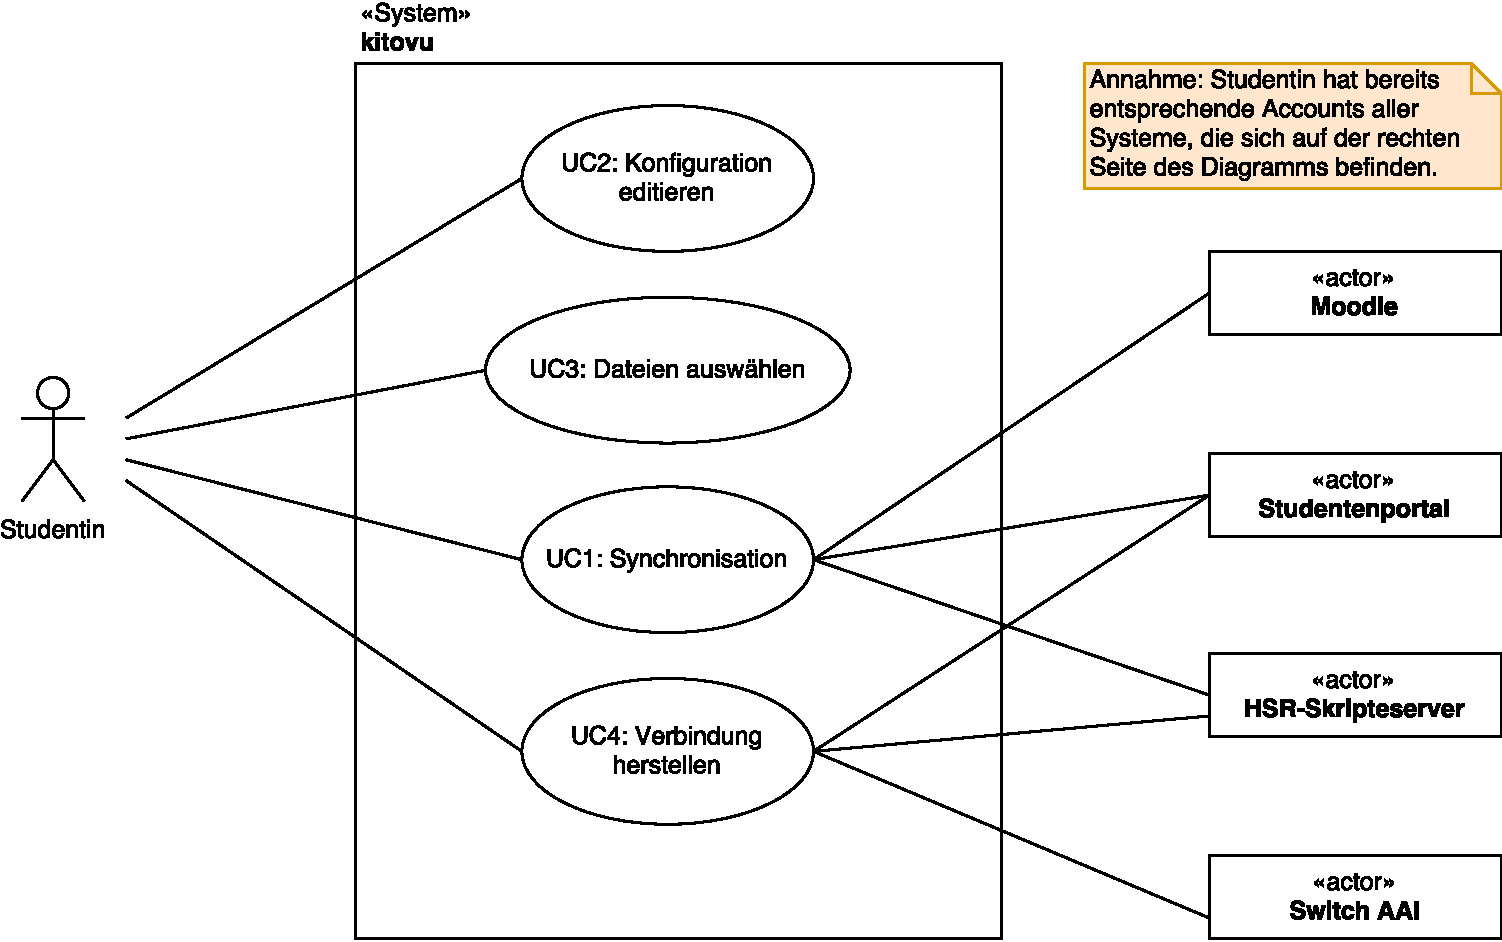
\includegraphics[width=40em]{./img/uc_diagram_kitovu.pdf}

\subsection{Beschreibungen (Brief)}
%<Alle Use Cases in einzelnen Kapiteln beschreiben im Brief Format>
\begin{description}
	
\item[Use Case 1: Synchronisation:] Die Studentin synchronisiert die Dateien von der externen Plattform auf ihren Rechner und hat sie danach offline verfügbar.
	
\item[Use Case 2: Konfiguration editieren:] Die Studentin legt in einer Konfigurationsdatei alle Plattformen und die entsprechenden Verbindungsdaten fest, mit der auf die externen Plattformen zugegriffen wird.

\item[Use Case 3: Dateien auswählen:] Die Studentin legt in der Konfigurationsdatei fest, welche Ordner und Dateien synchronisiert werden sollen.

\item[Use Case 4: Verbindung herstellen:] Die Studentin stellt eine Verbindung zur externen Plattform her und authentisiert sich dort.


\end{description}

\pagebreak
\subsection{Beschreibungen (Fully Dressed)}
%<Spezielle und wichtige Use Cases in einzelnen Kapiteln beschreiben im Fully Dressed Format>

\SetEnumitemKey{uclist}{labelwidth=13em,leftmargin=13.5em}
Da \emph{kitovu} keine grosse Komplexität aufweist, verwenden wir eine vereinfachte Version der ausführlichen ``Fully Dressed Use Cases'', wie sie beispielsweise Karl Wiegers beschreibt (vgl. ``Use Cases for Cafeteria Ordering System, Release 1.0'', 2002).


\subsubsection{UC1: Synchronisation der Dateien}

\begin{description}[uclist]
	\item[Goal] Die Studentin synchronisiert alle benötigten Unterrichtsmaterialien auf ihren Computer.
	\item[Primary Actor] Die Studentin
	\item[Trigger] Die Studentin möchte aktuelle Unterrichtsmaterialien auf ihrem Computer lokal abspeichern, so dass sie danach offline verfügbar sind.
	\item[Stakeholders and Interests]
	\begin{description}
		\item[Die Studentin] möchte stets die Version der Dateien auf ihrem Rechner haben, die sie tatsächlich will. Sie möchte offline mit ihnen arbeiten können, unabhängig von externen Plattformen.
		\item[Das System] stellt sicher, dass die gespeicherten Dateien konsistent und aktuell sind.
	\end{description}
	\item[Preconditions] UC4: Die Studentin hat erfolgreich eine Verbindung zur externen Plattform hergestellt.
	\item[Main Success Scenario] Die Studentin startet den Synchronisationsprozess. Danach verfügt sie über die von ihr ausgewählten Unterrichtsmaterialien auf ihrem Rechner. Eine Log-Ausgabe protokolliert den Vorgang.
	\item[Extensions]
	\begin{description}
		\item[Dateien schon vorhanden:] Die Studentin legt in ihrem Profil fest, wie mit bereits existierenden Dateien umgegangen werden soll. Dabei kann sie wählen, ob lokal bestehende Dateien gleichen Namens umbenannt, durch eine neuere Plattform-Version ersetzt oder nichts synchronisiert werden soll. Sie kann auch entscheiden, bei jedem Konflikt von \emph{kitovu} gefragt zu werden, wie sie für jede Datei entscheiden möchte.
		\item[Synchronisation schlägt fehl:] Die Synchronisation wird nicht durchgeführt, die Studentin erhält eine Benachrichtigung.
	\end{description}
	\item[Frequency of Occurrence] Rund jede Woche, wenn die Dozenten erneut neue Unterrichtsmaterialien bereitstellen.
\end{description}


\subsubsection{UC2: Konfiguration editieren}
\begin{description}[uclist]
  \item[Goal] Die Studentin editiert die Konfiguration, in der alle externen Plattformen aufgelistet sind.
  \item[Primary Actor] Die Studentin
  \item[Trigger] Die Studentin möchte eine externe Plattform in \emph{kitovu} einbinden, um deren Unterrichtsmaterialien auf ihrem Rechner lokal zur Verfügung haben.
  \item[Stakeholders and Interests]
    \begin{description}
      \item[Die Studentin] erfasst eine neue Plattform in der Konfiguration.
      \item[Das System] informiert die Studentin, welche Plattformen unterstützt werden und stellt sicher, dass die Plattform bereits als Plugin implementiert wurde.
    \end{description}
  \item[Preconditions] Die Studentin besitzt einen Account der externen Plattform mit entsprechenden Login-Daten.
  \item[Postconditions] Die aktualisierte Konfiguration wird gespeichert.
  \item[Main Success Scenario] In der Konfiguration hinterlegt die Studentin Angaben zu einer externen Plattform. Sie kann die Zugangsdaten erstellen, speichern, abändern oder das Profil ganz entfernen. Die eingegebenen Daten werden in \emph{kitovu} gespeichert.
  \item[Extensions] Die eingegebenen Daten sind ungültig. \emph{Kitovu} weist die Studentin darauf hin.
  \item[Frequency of Occurrence] Selten, nach Bedarf.
\end{description}

\subsubsection{UC3: Dateien auswählen}
\begin{description}[uclist]
  \item[Goal] Die Studentin schreibt in die Konfiguration, welche Dateien sie auf ihren Rechner synchronisieren möchte. Sie kann ausschliessen, welche Dateien nicht synchronisiert werden.
  \item[Primary Actor] Die Studentin
  \item[Trigger] Die Studentin möchte nur bestimmte Dateien und Ordner auf ihrem Rechner haben.
  \item[Stakeholders and Interests]
    \begin{description}
      \item[Die Studentin] weiss, welche Dateien sie synchronisieren möchte.
      \item[Das System] kann die entsprechenden Dateien lokalisieren.
    \end{description}
  \item[Preconditions]
    \begin{itemize}[leftmargin=1em]
      \item UC2 ist erfolgt: Die Studentin besitzt einen Account der externen Plattform. Sie hat bereits ein Profil der externen Plattform in der Konfiguration von \emph{kitovu} hinterlegt.
      \item Sie weiss, welche Dateien sie synchronisieren möchte und wo sie auf der externen Plattform abgelegt sind.
    \end{itemize}
  \item[Postconditions] Die aktualisierte Konfiguration wird gespeichert.
  \item[Main Success Scenario] Die Studentin definiert für das jeweilige Profil, welche Dateien sie synchronisiert haben möchte und welche ausgeschlossen werden.
  \item[Extensions] Die angegebenen Pfade existieren nicht -- die Studentin wird in UC1 darauf hingewiesen.
  %\item[Special Requirements]
  \item[Frequency of Occurrence] Zu Beginn jedes Semesters, wenn die neuen Module beginnen.
  %\item[Open Issues]
\end{description}

\subsubsection{UC4: Verbindung erstellen}
\begin{description}[uclist]
  \item[Goal] Um auf die Unterrichtsmaterialien zuzugreifen, muss die Studentin eine Verbindung zur externen Plattform herstellen.
  \item[Primary Actor] Die Studentin
  \item[Trigger] Die Studentin möchte auf eine externe Plattform zugreifen.
  \item[Stakeholders and Interests]
    \begin{description}
      \item[Die Studentin] weiss, von welcher Plattform sie welche Dateien möchte.
      \item[Das System] kann die Verbindung herstellen.
    \end{description}
  \item[Preconditions] Die Studentin hat in UC1 die Profildaten der externen Plattform hinterlegt.
  \item[Postconditions] Keine.
  \item[Main Success Scenario] Die Studentin verbindet sich zur externen Plattform, die Authentisierung ist erfolgreich.
  \item[Extensions]
    \begin{description}
      \item[Die Verbindung misslingt:] \strut \\[-1em]
        \begin{itemize}[leftmargin=1em]
          \item Nicht im HSR-Netz (HSR-Skripteserver): Die Verbindung misslingt, da sich die Studentin nicht im HSR-Netz befindet oder nicht per VPN verbunden ist.
          \item Moodle-Probleme: Der Zugriff auf Moodle misslingt aufgrund Plattform-spezifischer Probleme.
          \item Die hinterlegten Login-Daten sind nicht korrekt.
        \end{itemize}
      \item[Keine Login-Daten hinterlegt:] \emph{kitovu} fordert die Studentin auf, ihre Login-Daten einzugeben.
      \item[HSR-Skripteserver:] Die externe Plattform verlangt, dass sich die Studentin im HSR-Netz befindet oder bereits eine VPN-Verbindung zur Plattform aufgenommen hat.
    \end{description}
  \item[Special Requirements] Die Studentin verfügt über einen Account der externen Plattform.
  \item[Frequency of Occurrence] Rund jede Woche, wenn die Dozenten neue Unterrichtsmaterialien bereitstellen.
\end{description}


\section{Entwürfe zur Benutzeroberfläche}

Erstellt mit \emph{Balsamiq Mockups 3}.\footnote{\url{https://balsamiq.com/}}


	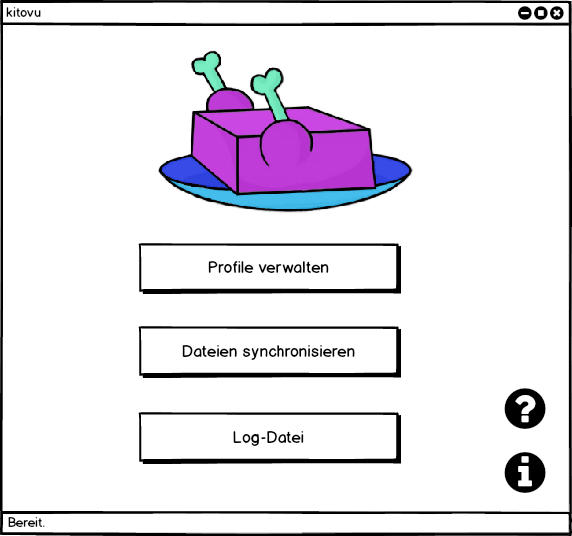
\includegraphics[width=30em]{./mockups/gui01.png}
	
	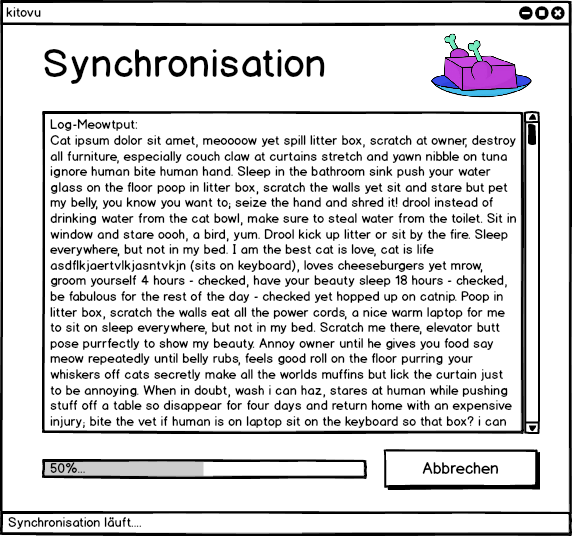
\includegraphics[width=30em]{./mockups/gui02.png}
	
	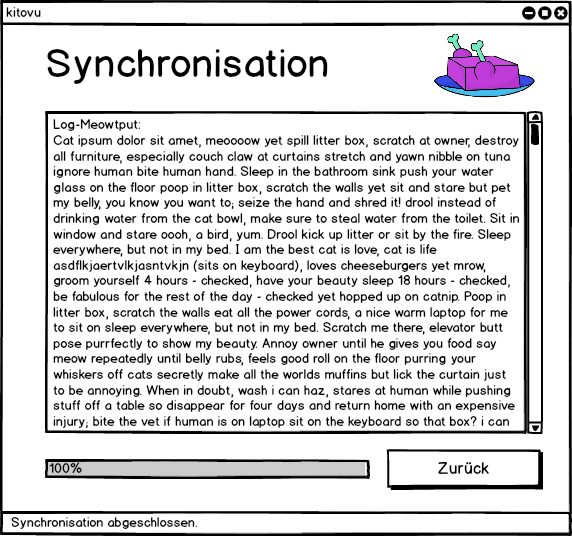
\includegraphics[width=30em]{./mockups/gui03.png}
	
	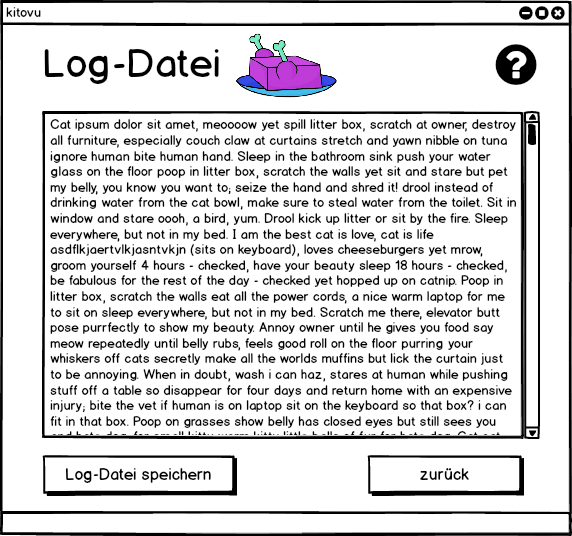
\includegraphics[width=30em]{./mockups/gui04.png}

	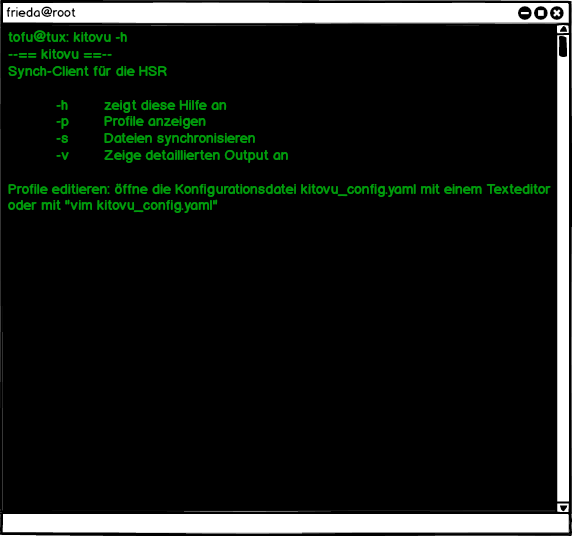
\includegraphics[width=30em]{./mockups/terminal01.png}
	
	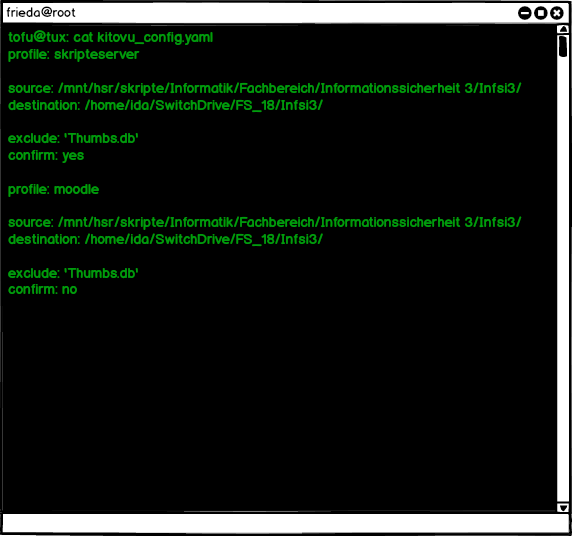
\includegraphics[width=30em]{./mockups/terminal02.png}
	
	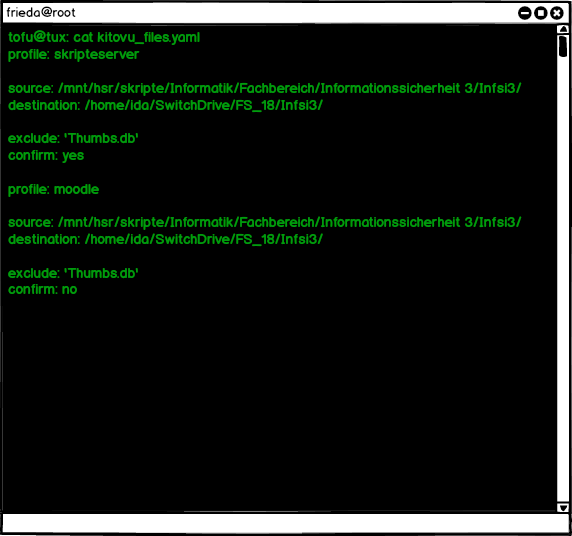
\includegraphics[width=30em]{./mockups/terminal03.png}
	
\section{Weitere Anforderungen}

\subsection{Qualitätsmerkmale}
%<Beschreibung der Qualitätsmerkmale der Software (Verweis auf ISO 9126 als Checkliste)>

\newcommand{\isourl}[2]{ISO/IEC #1\footnote{ISO/IEC #1 \url{https://www.iso.org/standard/#2.html}}}

Für die Qualitätsmerkmale haben wir uns für den Standard \isourl{9126}{16722} entschieden. Obwohl dieser bereits mit dem Standard \isourl{25010}{35733} überarbeitet wurde, verwenden wir die ältere Version, da wir damit im Modul \emph{Software-Engineering 1} bereits Erfahrung gesammelt haben.

Da das Projekt klein ist, haben wir nicht sämtliche Qualitätsmerkmale dieses Standards verwendet, sondern nur diejenigen, welche wir für \emph{kitovu} als passend empfunden haben.

\newcommand{\metricheader}[2]{\textbf{#1} & \textbf{#2}}

\subsubsection{Funktionalität (functionality)}

\begin{tabulary}{\linewidth}{lL}
  \toprule
  Metrik & Beschreibung \\
  \midrule

  \metricheader{1.1.}{Richtigkeit (accuracy)} \\
  1.1.1 & Eindeutig geänderte Dateien werden synchronisiert. Um geänderte Daten zu erkennen, sind wir auf die Angaben der Schnittstelle angewiesen. Wenn also die Schnittstelle nur ein Änderungsdatum zur Verfügung stellt, können wir nicht erkennen, ob die Datei zum angegebenen Änderungsdatum tatsächlich modifiziert wurde oder ob das Datum nachträglich entstanden ist. \\

  \metricheader{1.2.}{Ordnungsmässigkeit (regularity)} \\
  & \emph{Für die Ordnungsmässigkeit halten wir uns an das Bundesgesetz über den Datenschutz (DSG\footnotemark). Es wird nicht mit besonders schützenswerten Personendaten hantiert.} \\
  1.2.1. & Wir speichern die Daten immer nur auf dem Computer des Benutzers. \\
  1.2.2. & Die einzigen Daten, welche an Dritte gehen, sind die Anmeldedaten für die entsprechende Schnittstelle sowie die Namen der Dateien, welche synchronisiert werden müssen. \\
  1.2.3. & Sämtliche Änderungen an Daten werden von dem Benutzer ausgelöst. Durch die akkurate Benennung der Interaktionsmöglichkeiten macht \emph{kitovu} verständlich, welche Aktion der Benutzer auslöst. \\

  \metricheader{1.3.}{Sicherheit (security)} \\
  1.3.1. & \emph{Kitovu} legt Anmeldeinformationen wie Passwörter und Login-Tokens verschlüsselt auf dem System ab. \\
  1.3.2. & Die Ablage der synchronisierten Daten und Konfigurationen geschieht nicht verschlüsselt. Es liegt also in der Hand des Benutzers, vorsichtig damit umzugehen. \newline Falls vertrauliche Daten synchronisiert werden, muss der Benutzer sicherstellen, dass die von der externen Plattform synchronisierten Dateien nicht an einem Ort gespeichert werden, der für unbefugte Dritte zugänglich ist. \\
  \bottomrule
\end{tabulary}

\footnotetext{\url{https://www.admin.ch/opc/de/classified-compilation/19920153/index.html}}

\subsubsection{Zuverlässigkeit (reliability)}

\begin{tabulary}{\linewidth}{lL}
  \toprule
  Metrik & Beschreibung \\
  \midrule

  \metricheader{2.1.}{Fehlertoleranz (fault tolerance)} \\
  2.1.1. & Falls ein Modul fehlerhaft ausgeführt wird -- falls beispielsweise ein Server nicht erreichbar ist -- wird dies dem Benutzer mitgeteilt, aber sämtliche anderen Module werden ausgeführt. \\
  2.1.2. & Fehlerhafte Eingaben in der Konfiguration werden dem Benutzer verständlich kommuniziert. \\

  \metricheader{2.2.}{Wiederherstellbarkeit (recoverability)} \\
  2.2.1. & Falls eine Synchronisation nur zum Teil ausgeführt werden konnte, kann \emph{kitovu} die Synchronisation erneut ausführen und nur versuchen, die fehlenden Teile zu synchronisieren. \\
  2.2.2. & Falls sämtliche Dateien verloren gegangen sind, etwa bei einem Festplattendefekts, muss die Konfigurationsdatei erneut geschrieben werden. Um dem vorzubeugen, kann ein Backup der Konfigurationsdatei erstellt werden. \\
  \bottomrule
\end{tabulary}

\subsubsection{Benutzbarkeit (usability)}

\begin{tabulary}{\linewidth}{lL}
  \toprule
  Metrik & Beschreibung \\
  \midrule
  \metricheader{3.1.}{Verständlichkeit (understandability)} \\
  3.1.1 & Das Synchronisieren wird über eine übersichtliche grafische Oberfläche respektive mit der \verb|--help|-Option des Kommandozeilenprogramm beschreiben. \\
  3.1.2 & Die Konfiguration der einzelnen Profile erfolgt über eine separate Ansicht/Datei. \\
  \metricheader{3.2.}{Bedienbarkeit (operability)} \\
  3.2.1. & Wenn die Konfiguration erstellt ist und die Login-Daten gespeichert wurden, kann die eigentliche Synchronisation in höchstens zwei Schritten durchgeführt werden. \\
  3.2.2. & Falls die Login-Daten noch nicht eingegeben wurden, wird pro Modul ein weiterer Schritt benötigt. \\
  \bottomrule
\end{tabulary}

\subsubsection{Effizienz (efficiency)}

\begin{tabulary}{\linewidth}{lL}
  \toprule
  Metrik & Beschreibung \\
  \midrule
  \metricheader{4.1.}{Zeitverhalten (time behaviour)} \\
  & \emph{Das Zeitverhalten ist abhängig von den externen Schnittstellen und des eigenen Internetanschlusses.} \\
  4.1.1. & Pro Modul wird immer nur eine Anfrage abgesetzt, um herauszufinden, ob sich die Dateien auf der externen Plattform geändert haben. Je nach dem bietet die externe Schnittstelle keine solche Funktion, wodurch mehr Anfragen abgeschickt werden müssen. \\
  4.1.2. & Eine Analyse der bisherigen Unterrichtseinheiten zeigt,\footnote{Im Schulkontext ist das ein ``Modul'', jedoch führt dies zu Verwirrung mit unserer Bezeichnung von ``Modul'' für eine externe Plattform, die \emph{kitovu} einbindet.} dass pro Unterrichtseinheit über das ganze Semester verteilt ungefähr 1'000 Dateien synchronisiert werden. Dies bedeutet bei einer wöchentlichen Synchronisation mit 7 Einheiten jeweils: \[ 1'000~\frac{\textrm{Dateien}}{\textrm{Unterrichtseinheit}} * 7\ \textrm{Module} / 14\ \textrm{Wochen} = 500~\frac{\textrm{Dateien}}{\textrm{Woche}} \] \\ 
  \bottomrule
\end{tabulary}

FIXME Florian: Fussnote 10 einbinden.

\subsubsection{Änderbarkeit (maintainability)}

\begin{tabulary}{\linewidth}{lL}
  \toprule
  Metrik & Beschreibung \\
  \midrule
  \metricheader{5.1.}{Analysierbarkeit (analyzability)} \\
  5.1.1. & Mit einem Debug-Modus können zusätzlich alle Informationen, die ein Modul liefert, aufgezeichnet werden. Dies ermöglicht eine Einschränkung des Problems auf entweder ein spezifisches Modul oder den Kern-Teil von \emph{kitovu} selber. \\
  \metricheader{5.2.}{Modifizierbarkeit (changeability)} \\
  5.2.1. & Da die ganze Applikation modular aufgebaut ist, lässt sich diese leicht um neue Module erweitern oder reduzieren. \\
  \metricheader{5.3.}{Stabilität (stability)} \\
  5.3.1. & Die Test-Coverage ist mindestens 90\%. \\
  \metricheader{5.4.}{Prüfbarkeit (testability)} \\
  5.4.1. & Dank des modularen Aufbaus werden alle Module und der Kern-Teil separat getestet. \\
  \bottomrule
\end{tabulary}

\subsubsection{Übertragbarkeit (portability)}

\begin{tabulary}{\linewidth}{lL}
  \toprule
  Metrik & Beschreibung \\
  \midrule
  \metricheader{6.1.}{Installierbarkeit (installability)} \\
  6.1.1. & Die Applikation lässt sich über ein pip-Paket\footnotemark{} installieren. \\
  6.1.2. & Für Windows (und allenfalls macOS) wird \emph{kitovu} als ausführbare Datei bereitgestellt. Diese installiert sämtliche Abhängigkeiten mit. \\
  \bottomrule
\end{tabulary}
\footnotetext{\url{https://pypi.python.org/pypi/pip}}

\subsection{Schnittstellen}
%<Beschreibung der Schnittstellen der Software>

Folgende Schnittstellen werden im Projekt \emph{kitovu} zu Verfügung gestellt oder verwendet:

\begin{description}
  \item[Grafische Benutzeroberfläche]
    Die grafische Benutzeroberfläche ist die Schnittstelle, mit der die meisten Endbenutzer mit der Applikation interagieren.
    Diese bietet einen einfachen Weg, um die Daten zu synchronisieren.
  \item[Kommandozeilenprogramm]
    Alternativ bieten wir ein Kommandozeilenprogramm an, welches über einfache Befehle die Synchronisation startet.
    Dies ist besonders für die Automatisierung gedacht oder für Endbenutzer, welche die Kommandozeile bevorzugen.
  \item[Externe Schnittstellen ("Plugins")]
    Wir verwenden als externe Schnittstellen das Studentenportal, das Moodle und den Skripteserver sowie das Switch AAI für die Moodle-Autorisierung.
\end{description}

\subsection{Randbedingungen}
%<Auflistung der wichtigsten Randbedingungen mit einer Beschreibung dazu>

Diese technischen Randbedingungen wurden für das Projekt \emph{kitovu} festgelegt:

\begin{description}
  \item[Python] Version 3.6
  \item[Betriebssystem] \emph{kitovu} unterstützt Windows und Linux, gegebenfalls macOS. Weitere technische Randbedingungen sind im Projektplan aufgeführt.
\end{description}
\end{document}
